\documentclass{acm_proc_article-sp}
\usepackage{url}
\usepackage{booktabs}
\usepackage{multirow}
\usepackage{graphicx}
\begin{document}
% --- Author Metadata here ---
%\conferenceinfo{PCSC02}{Manila, Philippines}
%\setpagenumber{50}
%\CopyrightYear{2002} % Allows default copyright year (1999) to be over-ridden - IF NEED BE.
%\crdata{0-12345-67-8/90/01}  % Allows default copyright data (0-89791-88-6/97/05) to be %over-ridden - IF NEED BE.
% --- End of Author Metadata ---
\title{AI201 PA 2 Report\\ Naive Bayes Spam Filter}

\numberofauthors{1}
\author{
\alignauthor John Louis D. Lagramada (2025-22174)\\ % your name and student number
~\\
Date of Submission: March 6, 2025
}
% Define \@copyrightspace if the class omitted it (prevents \maketitle error)
\makeatletter
\@ifundefined{@copyrightspace}{\def\@copyrightspace{}}{}
\makeatother

\maketitle


\section{Introduction}

Electronic mail or email have revolutionized the way we communicate from traditional mail. However, it gave rise to unsolicited emails called spam that may contain dangerous content, advertisements, or scams.
There is a need to develop a technology that can filter out these spam emails automatically, while keeping the legitimate emails intact. This presents a challenge as the emails contain a wide breadth of content such as text, images, HTML, and attachments. In this study, we focused on classifying emails based on their text content.

We developed machine learning models that can classify emails as either spam or ham (legitimate) emails. These models are based on the Naive Bayes algorithm which we extend with the Lambda smoothing technique. Additionally, we adopted the mutual information technique as documented by Hovold (2006).

We evaluated the performance of these methods in a subset of the TREC06 corpus dataset and analyzed the results based on the model's precision, recall, F1 score, and the receiver operating characteristic (ROC) curve. The models are implemented minimally in Python and follows the standards for classical machine learning models.

\section{Objectives}
The objectives of this study is to develop a Naive Bayes classifier for spam filtering and to investigate the effects of Lambda smoothing and mutual information feature selection on the performance of the model and time and space complexities. Specifically, we aim to achieve the following objectives:
\begin{enumerate}
    \item Investigate the performance of the Naive Bayes classifier in classifying emails as either spam or ham.
    \item Determine the effects of Lambda smoothing and find the optimal value for $\lambda$ that produces the best model performance.
    \item Analyze the effects of feature selection via mutual information with different values of $k$ and find the optimal value for $k$ that produces the best model performance.
    \item Lastly, this study aims to analyze the tradeoff between computational/memory cost and model performance and the tradeoff between precision and recall to explain what works best for spam filtering.

\end{enumerate}

\section{Methodology}
We investigated the performance of the base Naive Bayes classifier, Lambda smoothed Naive Bayes classifier, and mutual information feature selection. We split the dataset into a 70-30 train-test split and evaluated the performance of each of the models discussed. We used accuracy, precision, recall, and F1 score as our evaluation metrics and chose the best performing model based on the receiver operating characteristic (ROC) curve.

\subsection{Naive Bayes Classifier}
The Naive Bayes classifier is a probabilistic algorithm that is given by,
\begin{equation}
    P(\omega|\mathbf{x})=\frac{\prod_{i=1}^d{P(x_i|\omega)P(\omega)}}{\sum_\omega\prod_{i=1}^d{P(x_i|\omega)P(\omega)}}
\end{equation}

where $P(\omega|\mathbf{x})$ is the posterior probability that a vector of unique words $\textbf{x}$ drawn from the email belongs to class $\omega$, $P(x_i|\omega)$ is the conditional class likelihood of the word $x_i$ belonging in class $\omega$, and $P(\omega)$ is the prior distribution that an email belongs to class $\omega$.
The Naive Bayes classifier assumes that $P(x_i|\omega)$ is independent of the probability $P(x_j|\omega)\  \forall i \neq j$.

The spam filter classifies an email as either legitimate (ham) or unsolicited (spam), making it a binary classifier. We can express the Naive Bayes classifier for these two classes where $\omega \in \{h, s\}$ as,
\begin{equation}
    P(h|\mathbf{x})=\frac{\prod_{i=1}^d{P(x_i|h)P(h)}}{\prod_{i=1}^d{P(x_i|h)P(h)}+\prod_{i=1}^d{P(x_i|s)P(s)}}
\end{equation}

The class conditional likelihood $P(x_i|\omega)$ is estimated as follows,
\begin{equation}
    P(x_i|\omega) = \frac{\sum_{D\in D_\omega} I(x_i\in D)}{|D_\omega|}
\end{equation}
where $D_\omega$ is the set of emails in class $\omega$, and $I(x_i\in D)$ is an indicator function that returns 1 if the word $x_i$ is present in email $D$, and 0 otherwise.

To avoid arithmetic underflow, the logarithm of each term is taken and summed altogether to compute for the posterior probability. Algorithmically, the Naive Bayes classifier can be expressed as follows for $\omega \in \{h, s\}$,
$$
    \mathcal{P}(\omega) = \prod^d_{i=1}P(x_i|\omega)P(\omega) = e^{\ln{P(\omega)}+\sum_{i=1}^d\ln{P(x_i|\omega)}}
$$
\begin{equation}
    P(h|\mathbf{x}) = \frac{\mathcal{P}(h)}{\mathcal{P}(h)+\mathcal{P}(s)} 
\end{equation}

Since $\ln\mathcal{P}(\omega)$ is bounded by $(-\infty, 0]$ and finite computer precision may cause it to underflow for largely negative values, we can compute the posterior probability using the shift trick as follows,
\begin{equation}
P(h|\mathbf{x}) = \frac{e^{\ln\mathcal{P}(h) - M}}{e^{\ln\mathcal{P}(h) - M} + e^{\ln\mathcal{P}(s) - M}}
\end{equation}
where $M = \max\{\ln\mathcal{P}(h), \ln\mathcal{P}(s)\}$, forcing the largest term to be zero and the smaller term be easily calculated without the risk of underflow.

The Naive Bayes classifier diverges when $P(x_i|\omega) = 0$ for any word $x_i$ in the email. In this paper, we initially represented these cases with a probability of $-\infty$. We obtained this by getting the limit of $\ln{P(x_i|\omega)}$ as $P(x_i|\omega)$ approaches 0 from the right. This serves as the baseline of the other models.\footnote{This results for the model without Lambda smoothing. This isn't recommended but is required in the assignment, so we are forced to do this to avoid numerical instability.}
\subsection{Lambda Smoothing}
Collapsing the probability of $P(x_i|\omega) = 0$ to $-\infty$ logarithmically is not ideal as it causes the entire calculation to diverge. To address this, Lambda smoothing can be applied to the class conditional likelihoods as follows,
\begin{equation}
    P(x_i|\omega) = \frac{\sum_{D\in D_\omega} I(x_i\in D) + \lambda}{|D_\omega| + \lambda |V|}
\end{equation}
where $\lambda$ is the smoothing parameter, and $|V|$ is the vocabulary size. Laplace smoothing is a special case where $\lambda = 1$. With Lambda smoothing, $P(x_i|\omega) > 0$ even if the word didn't appear in the vocabulary, preventing it from diverging. We will investigate the effects of $\lambda$ on the precision and recall of the model and find the best model with the optimal $\lambda$.

\subsection{Mutual Information}
Naive Bayes classifier strongly assumes the independence of the words in the email. However, this is not usually the case as words may be correlated with each other. Large language models are built on this idea of word correlation called self-attention. To implement this in our simple Naive Bayes classifier, we can use Mutual Information (MI) to select the top $k$ words that are most correlated with the class labels. The mutual information of a word $x_i$ and class $\omega$ is given by,
\begin{equation}
    I(x_i; \omega) = \sum_{x_i\in\{0, 1\}}\sum_{\omega\in\{h, s\}} P(x_i, \omega) \log\frac{P(x_i, \omega)}{P(x_i)P(\omega)}
\end{equation}
where the double summation suggests that we take into account both the presence and absence of the word in either class. With this, we can save much more memory as we can limit our vocabulary with the top $k$ words with the highest mutual information. We will investigate the effects of $k$ on the precision and recall of the model and also the computational advantages of this method.

\section{Experimental Results}
We evaluated the performance of the Naive Bayes classifier models using precision, recall, F1 score, and the receiver operating characteristic (ROC) curve. These metrics are commonly used in classifier models to determine its performance across different classes. The best model selection  primarily is dependent on the area under the ROC curve (AUC) along with the F1-score which shows the model with the best precision and recall. However, in some cases, we focus on the recall of the model to minimize the number of true positive class (ham) being misclassified as negative class (spam).

We define these metrics as,

\begin{equation}
    \text{Precision} = \frac{\text{TP}}{\text{TP} + \text{FP}}
\end{equation}

\begin{equation}
    \text{Recall} = \frac{\text{TP}}{\text{TP} + \text{FN}}
\end{equation}

\begin{equation}
    \text{F1 Score} = 2 \cdot \frac{\text{Precision} \cdot \text{Recall}}{\text{Precision} + \text{Recall}}
\end{equation}

\begin{equation}
    \text{AUC} = \int_0^1 TPR(FPR) dFPR
\end{equation}

where $TP$ is the number of true positives, $FP$ is the number of false positives, $FN$ is the number of false negatives, and $TPR$ and $FPR$ are the true positive rate and false positive rate respectively. The positive class is the spam class, while the negative class is the ham class.

\subsection{Base Naive Bayes Results}
By collapsing the probabilities to $-\infty$ for the cases where $P(x_i|\omega) = 0$, we obtained the model performance metrics shown in Table 1. The model performs decently with a high precision and recall, serving as our benchmark before applying smoothing and mutual information techniques. 
\begin{table}[h]
\centering
\caption{Performance of Base Naive Bayes Classifier}
\begin{tabular}{lrr}
\toprule
Metrics & Score \\
\midrule
Precision & 0.93 \\
Recall & 0.89 \\
F1-Score & 0.91 \\
Accuracy & 0.94 \\
\bottomrule
\end{tabular}
\end{table}

\subsection{Lambda Smoothing Results}
Figure 1 shows the precision-recall tradeoff for different values of $\lambda$ in Lambda smoothing. We can see that as $\lambda$ increases, the precision increases while the recall decreases. The precision and recall scores also intersected at $\lambda = 8$.
\begin{figure}[h]
    \centering
    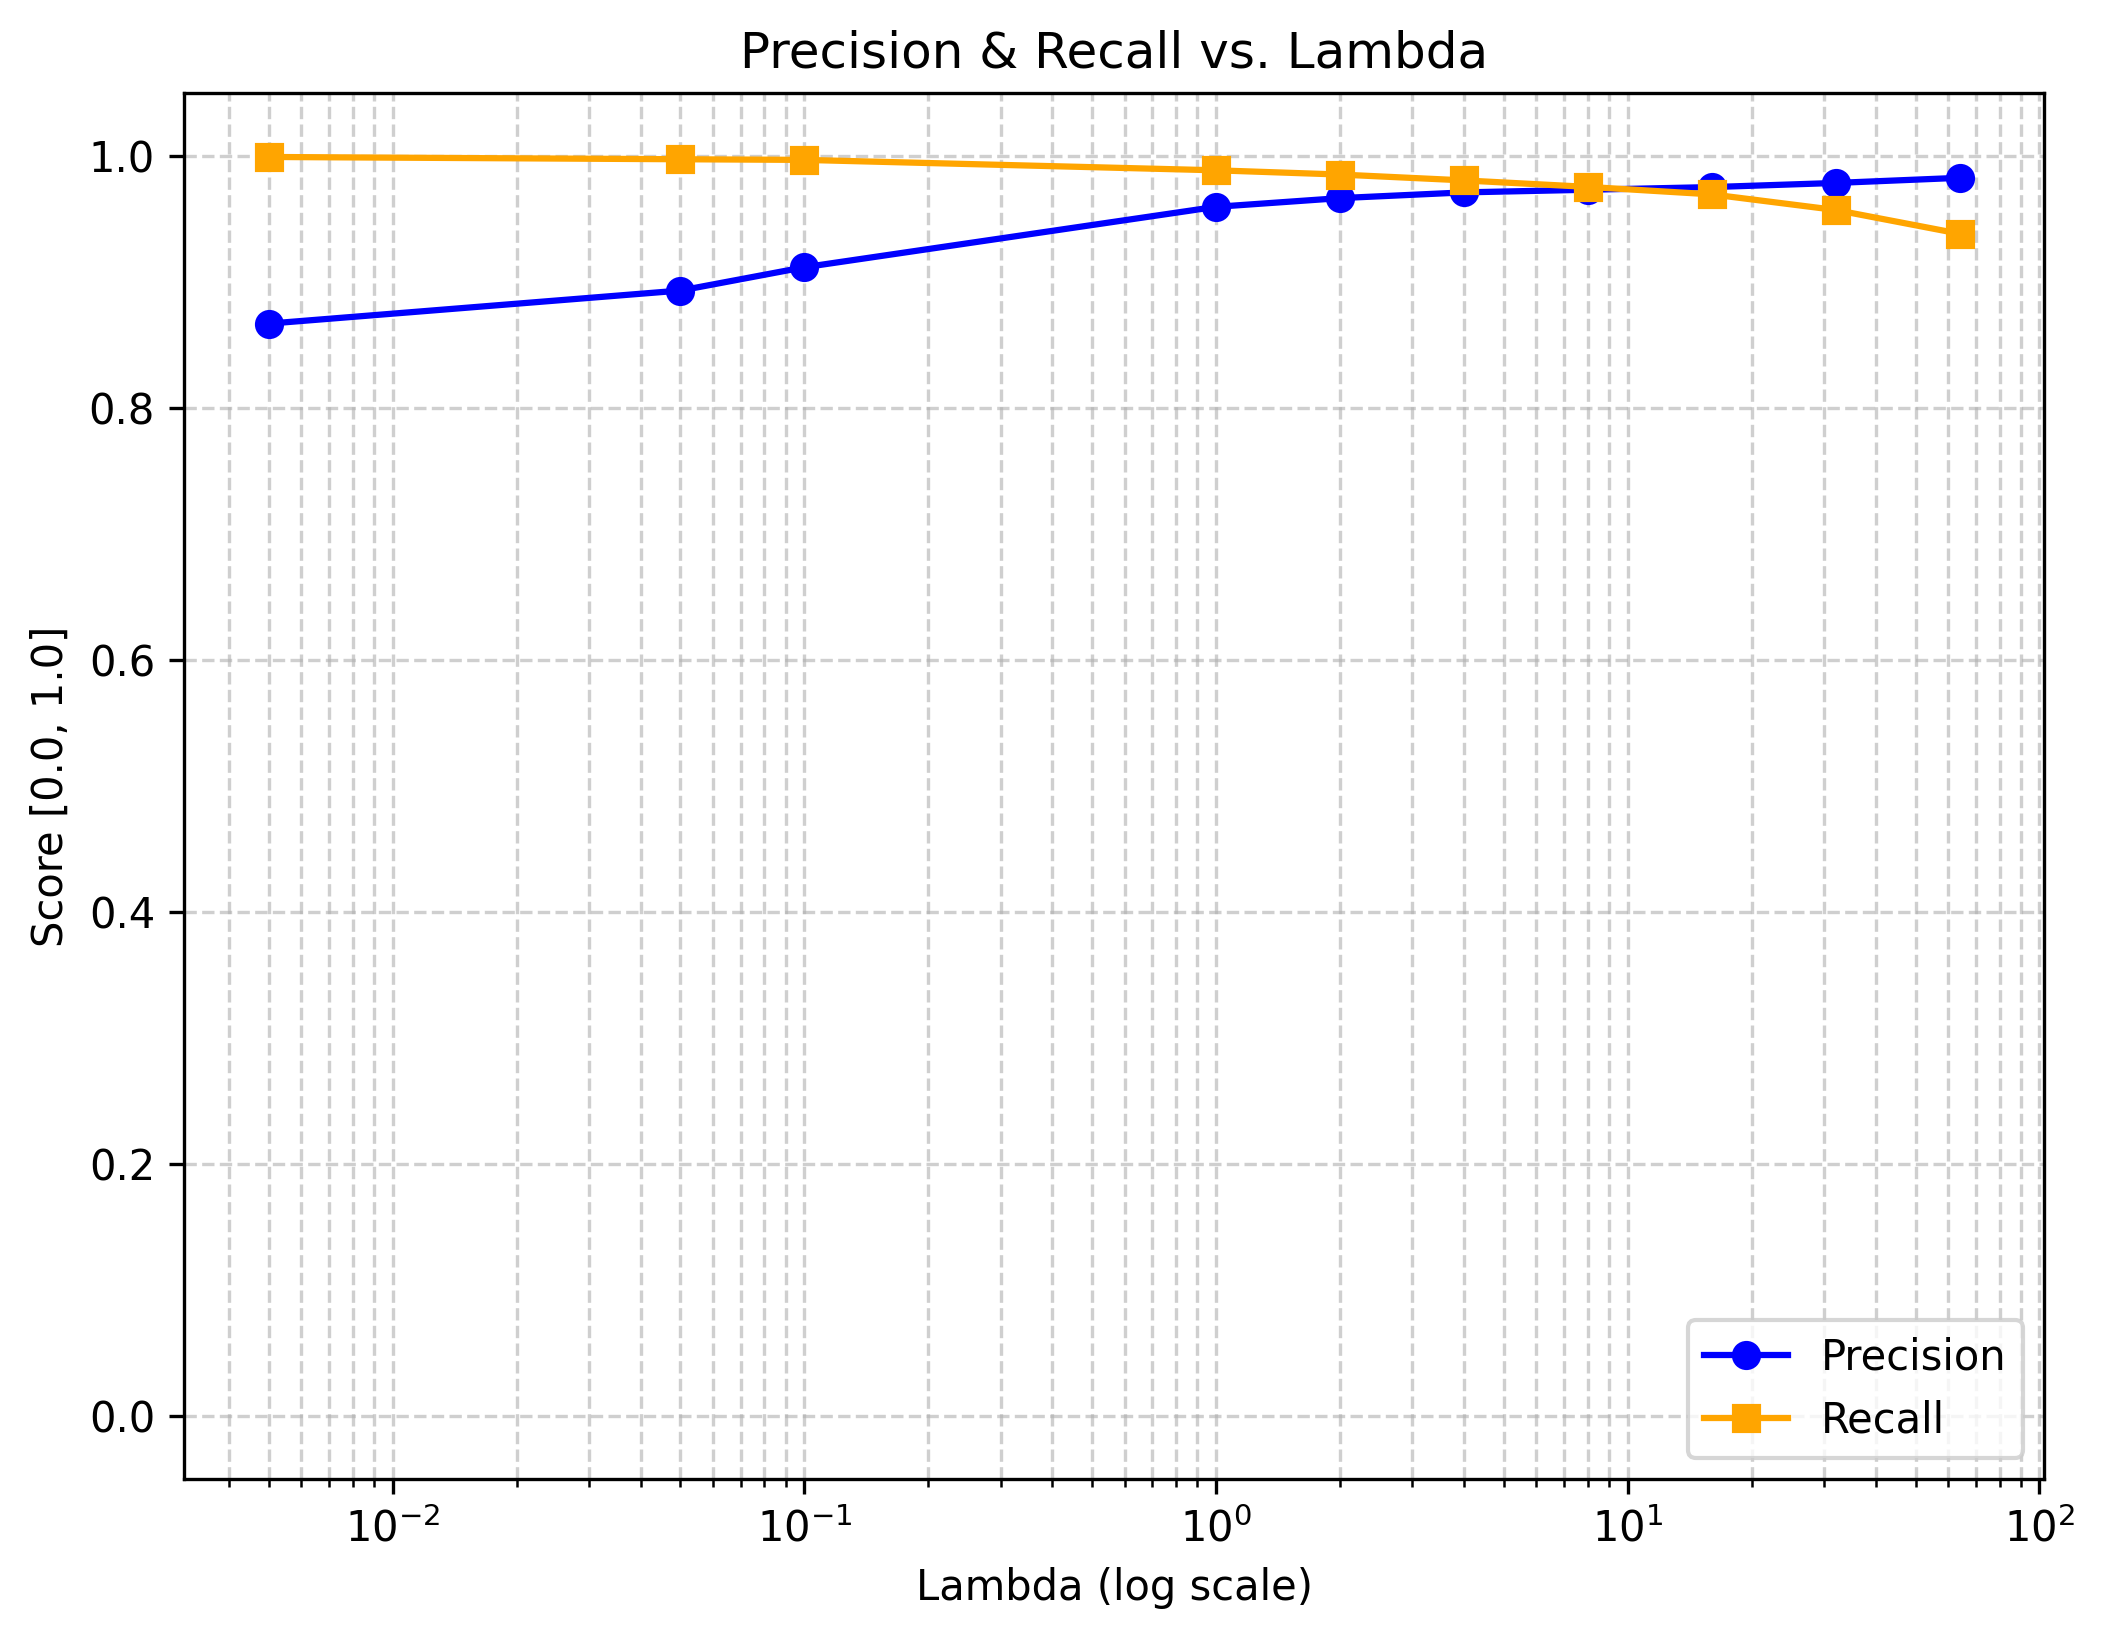
\includegraphics[width=0.475\textwidth]{results/precision_recall_tradeoff.png}
    \caption{Precision-Recall Tradeoff for Lambda Smoothing with different $\lambda$ values.}
    \label{fig:precision-recall}
\end{figure}


Figure 2 shows the F1-scores for different values of $\lambda$. The F1-score peaked at $\lambda = \{2.0,\ 4.0\}$ as it increases from $\lambda =0.005$. It then starts to decrease as $\lambda$ increases further.
\begin{figure}[h]
    \centering
    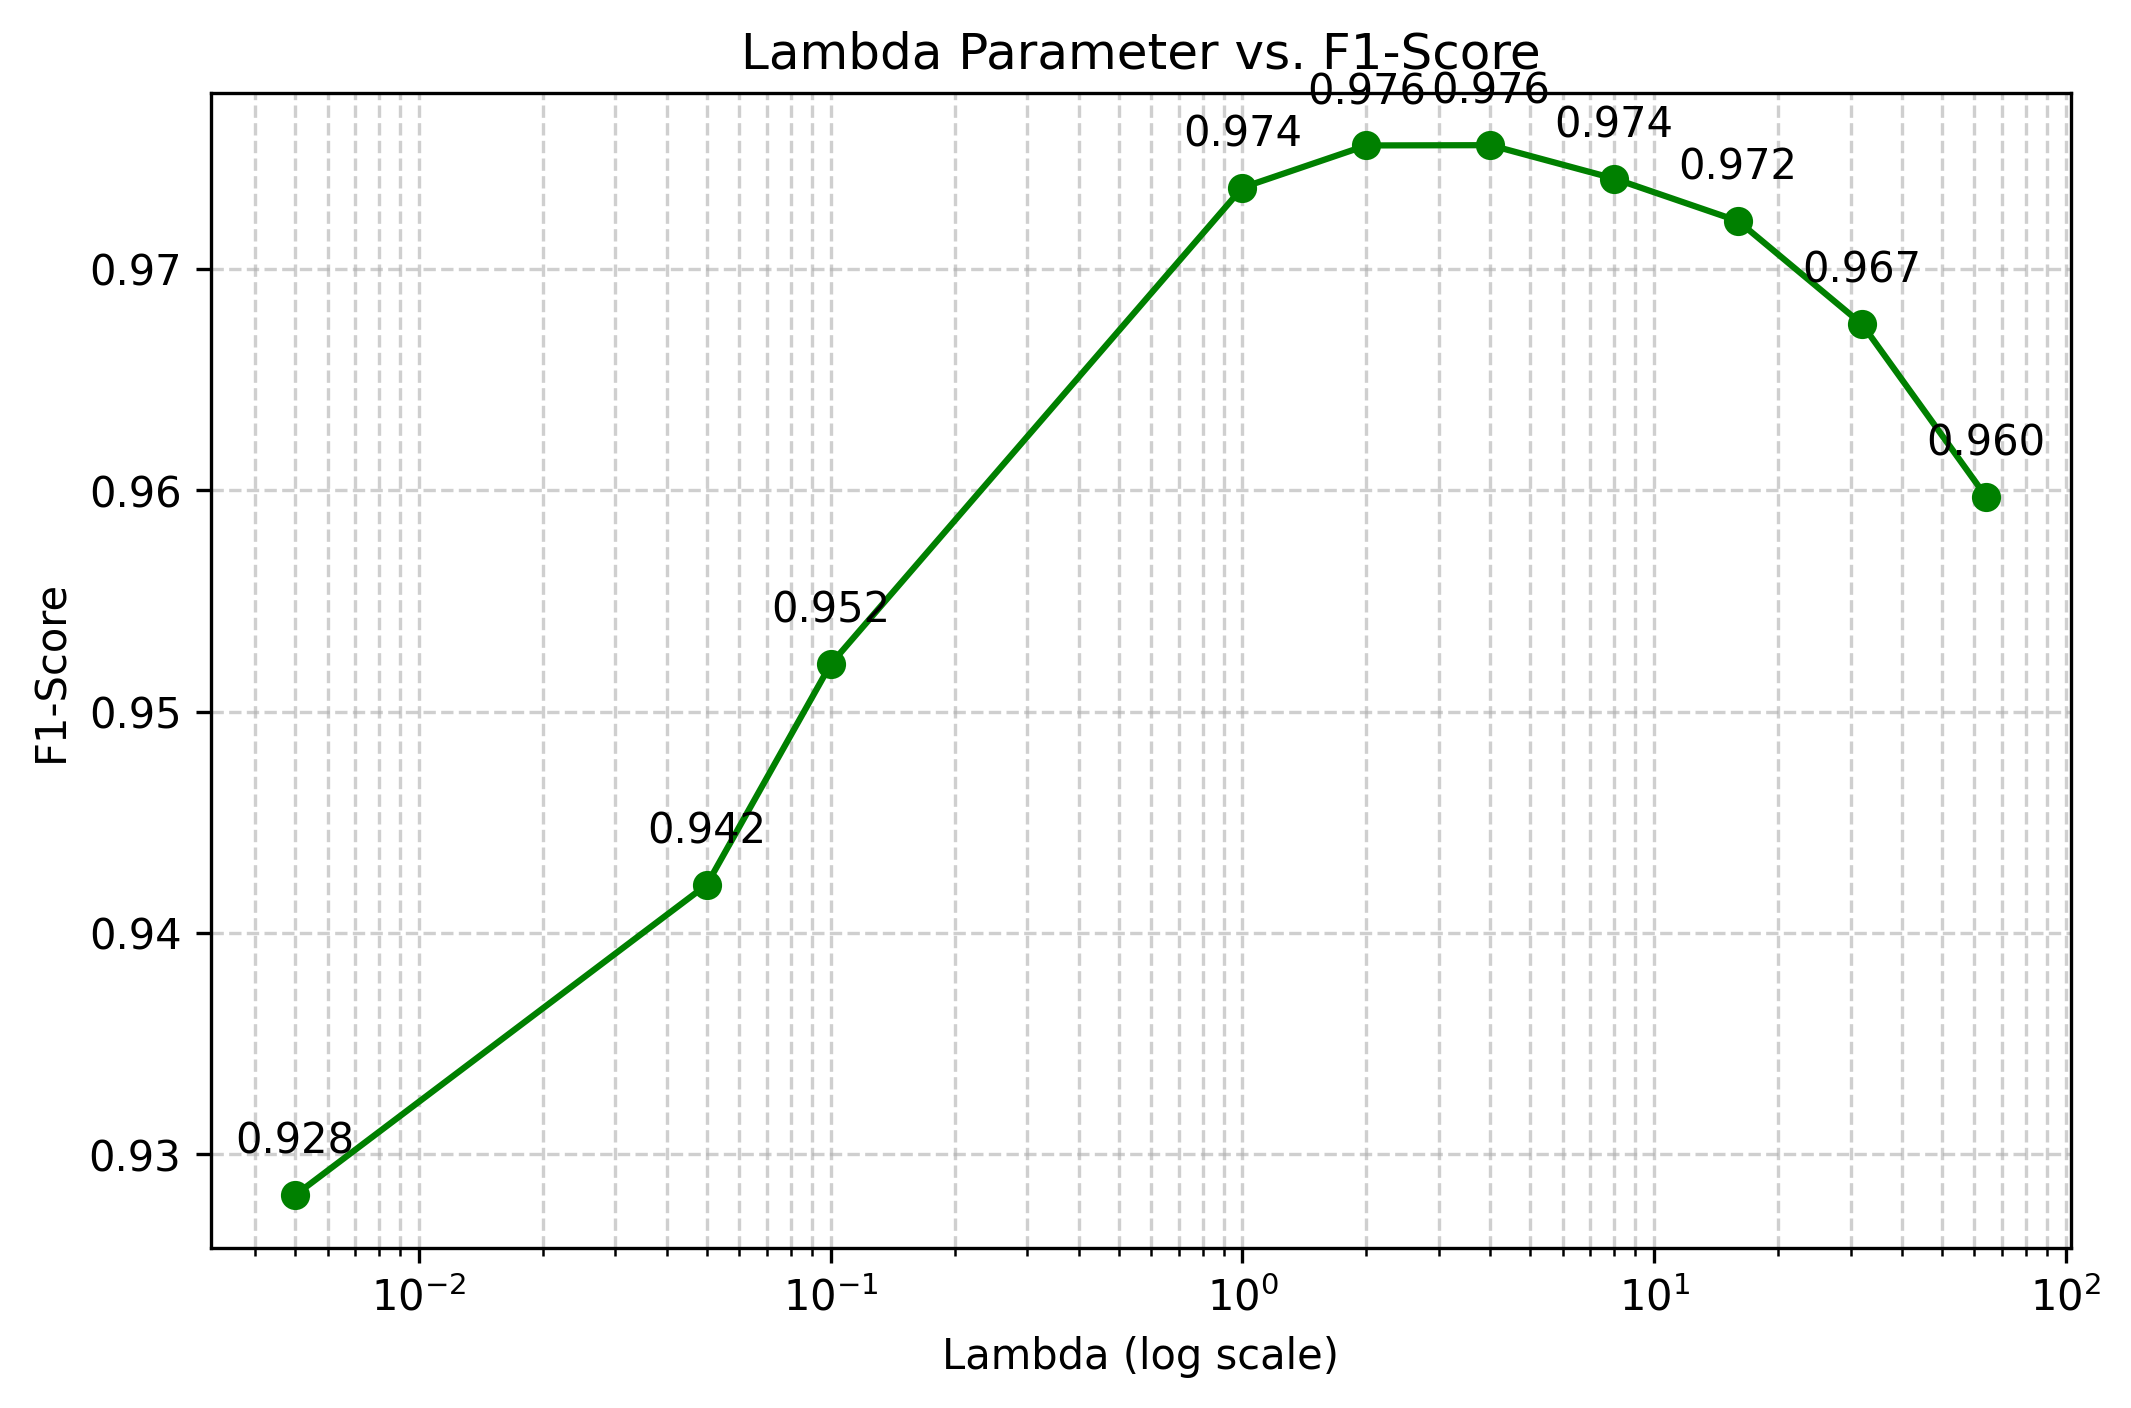
\includegraphics[width=0.475\textwidth]{results/lambda_vs_f1.png}
    \caption{F1-Scores for Lambda Smoothing with different $\lambda$ values.}
    \label{fig:f1-scores}
\end{figure}

Figure 3 shows the ROC curve for different values of $\lambda$. The same trend can be observed as with the F1-scores where the AUC peaked at $\lambda = \{2.0,\ 4.0\}$ that decreases as we further increase or decrease $\lambda$ from this interval.

\begin{figure}[h]
    \centering
    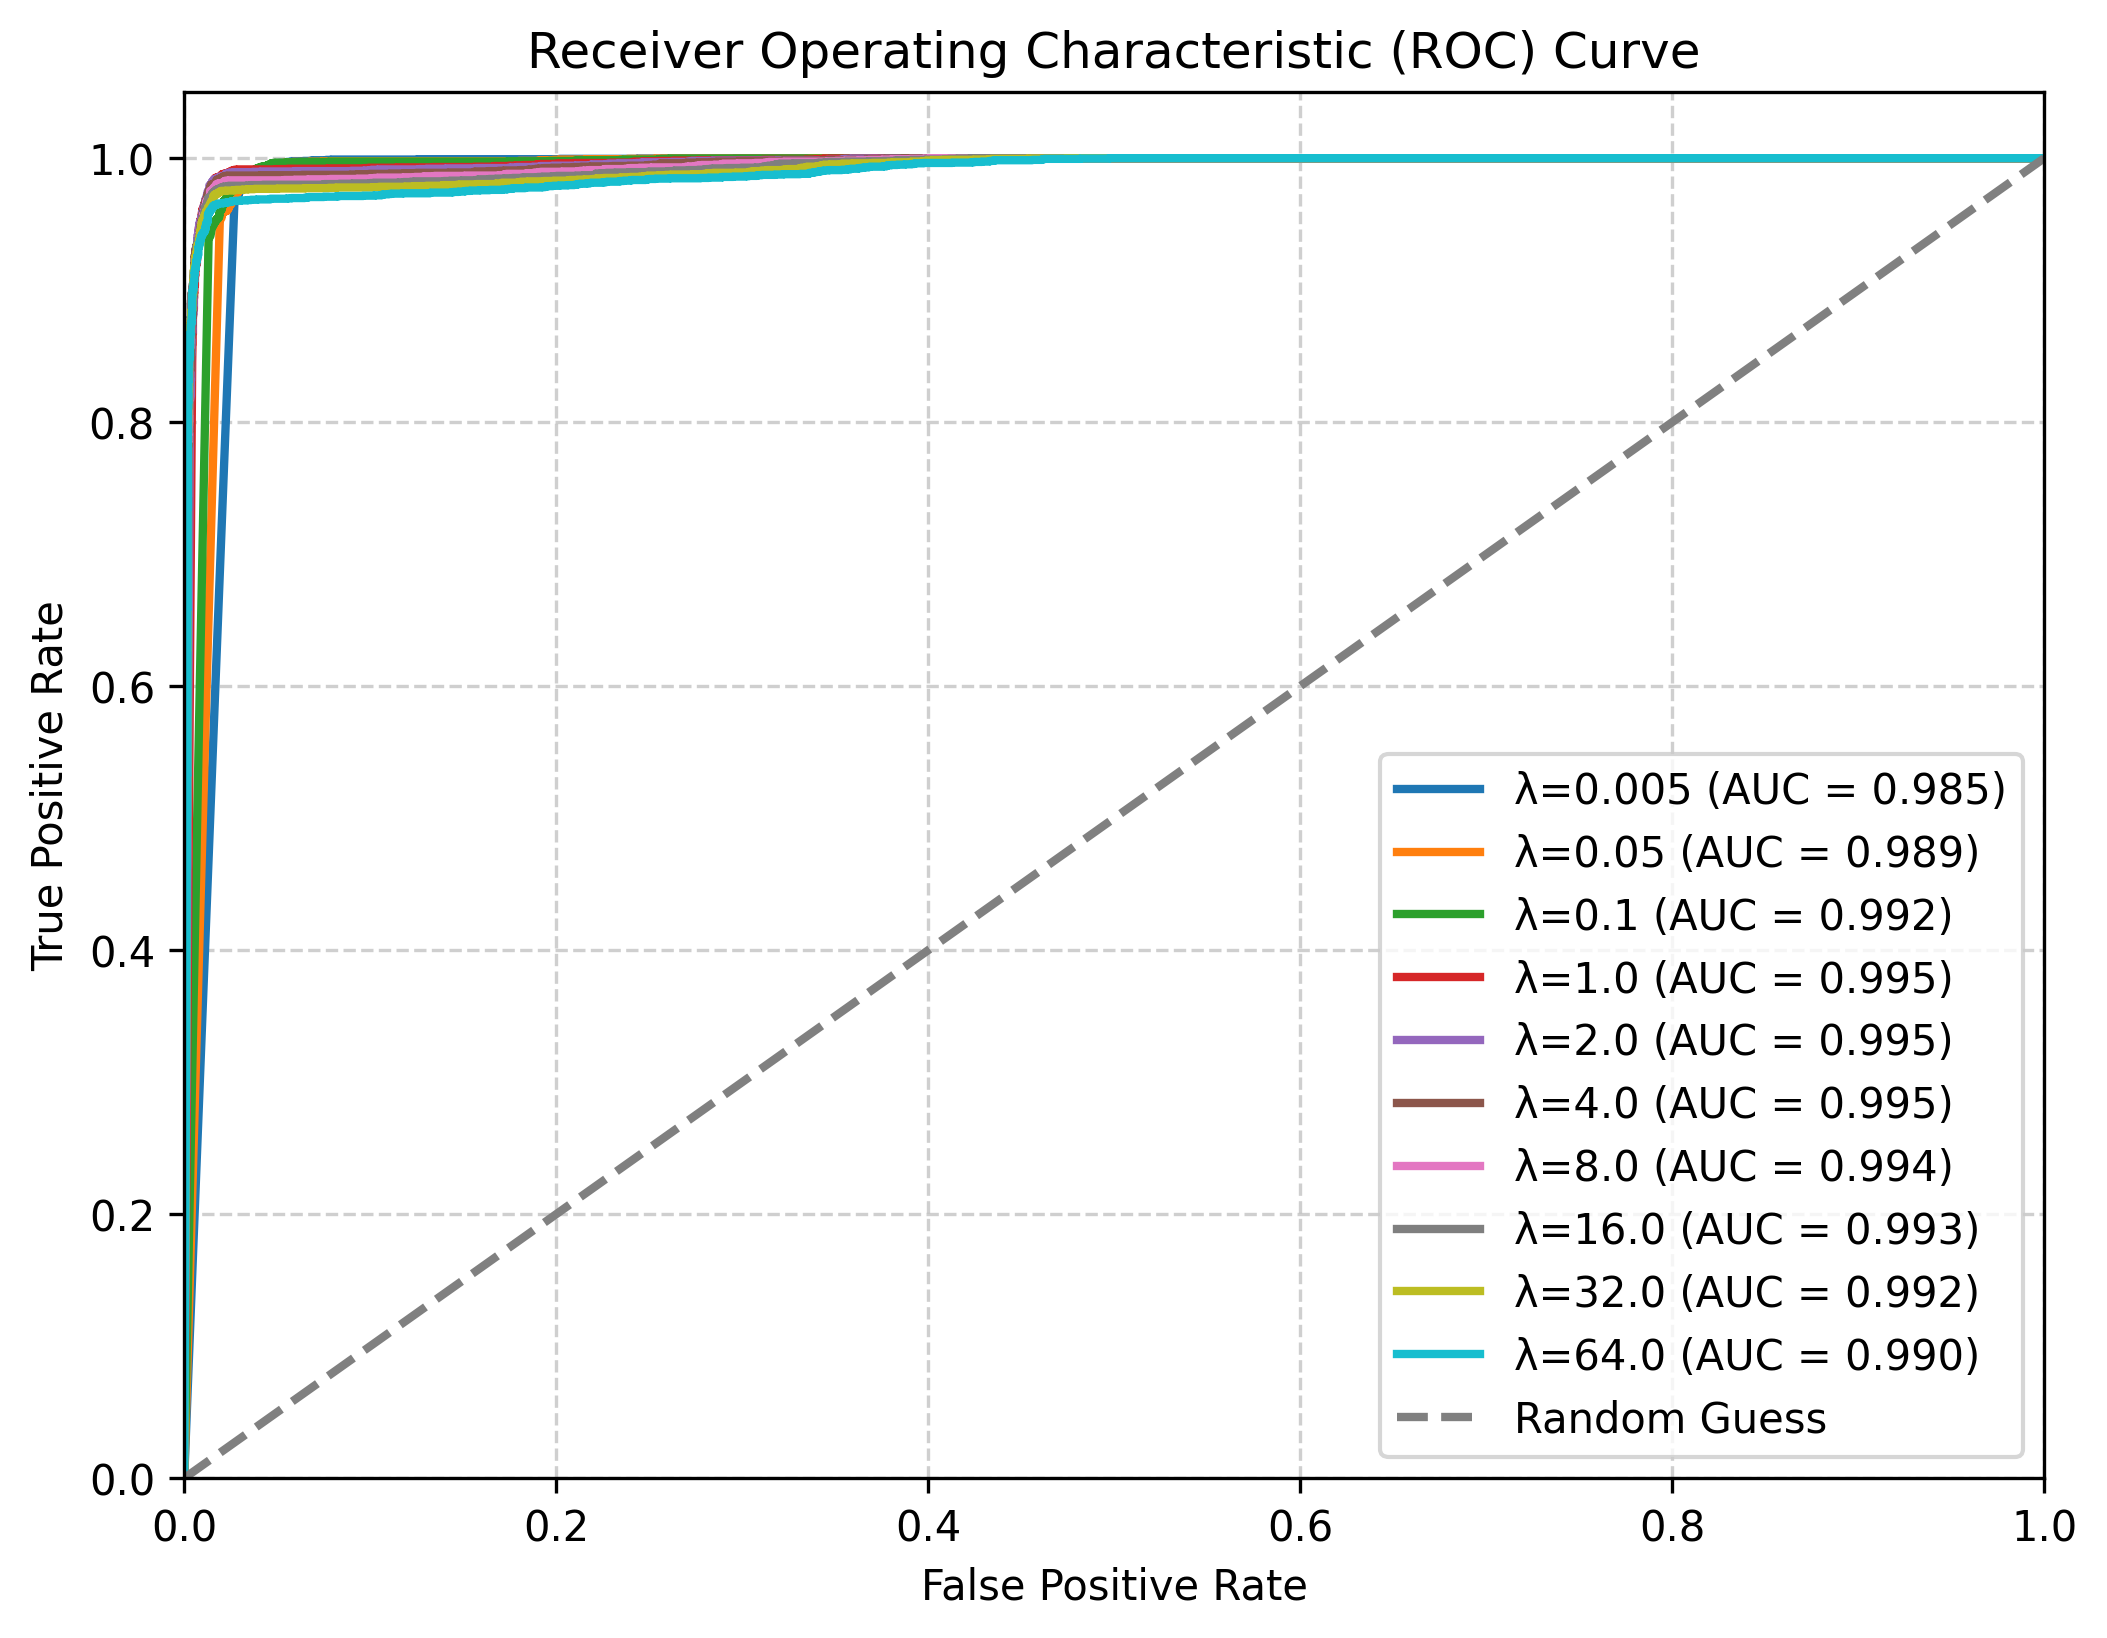
\includegraphics[width=0.475\textwidth]{results/roc_curve.png}
    \caption{ROC Curve for Lambda Smoothing with different $\lambda$ values.}
    \label{fig:roc-curve}
\end{figure}

Table 2 shows the raw performance metrics of the Lambda smoothing model with the different $\lambda$ values. From here, we chose $\lambda = 4.0$ as the best model and used it as the baseline for the mutual information feature selection model.

\begin{table}[h]
\centering
\caption{Comparison of Naive Bayes Performance with Varying $\lambda$}
\begin{tabular}{ccccc}
\toprule
$\lambda$ & Accuracy & Precision & Recall & F1-Score \\
\midrule
0.005 & 0.947 & 0.867 & 0.999 & 0.928 \\
0.050 & 0.958 & 0.893 & 0.997 & 0.942 \\
0.100 & 0.966 & 0.911 & 0.997 & 0.952 \\
1.000 & 0.982 & 0.959 & 0.988 & 0.974 \\
2.000 & 0.983 & 0.966 & 0.985 & 0.976 \\
4.000 & 0.983 & 0.971 & 0.980 & 0.976 \\
8.000 & 0.982 & 0.973 & 0.975 & 0.974 \\
16.000 & 0.981 & 0.975 & 0.969 & 0.972 \\
32.000 & 0.978 & 0.978 & 0.957 & 0.967 \\
64.000 & 0.973 & 0.982 & 0.938 & 0.960 \\
\bottomrule
\end{tabular}
\end{table}

Figure 4 shows the confusion matrix of the model with the optimal $\lambda$ value. We can see that the model performs well in classifying both ham and spam emails, with a high number of true positives and true negatives, and a low number of false positives and false negatives.

\begin{figure}[h]
    \centering
    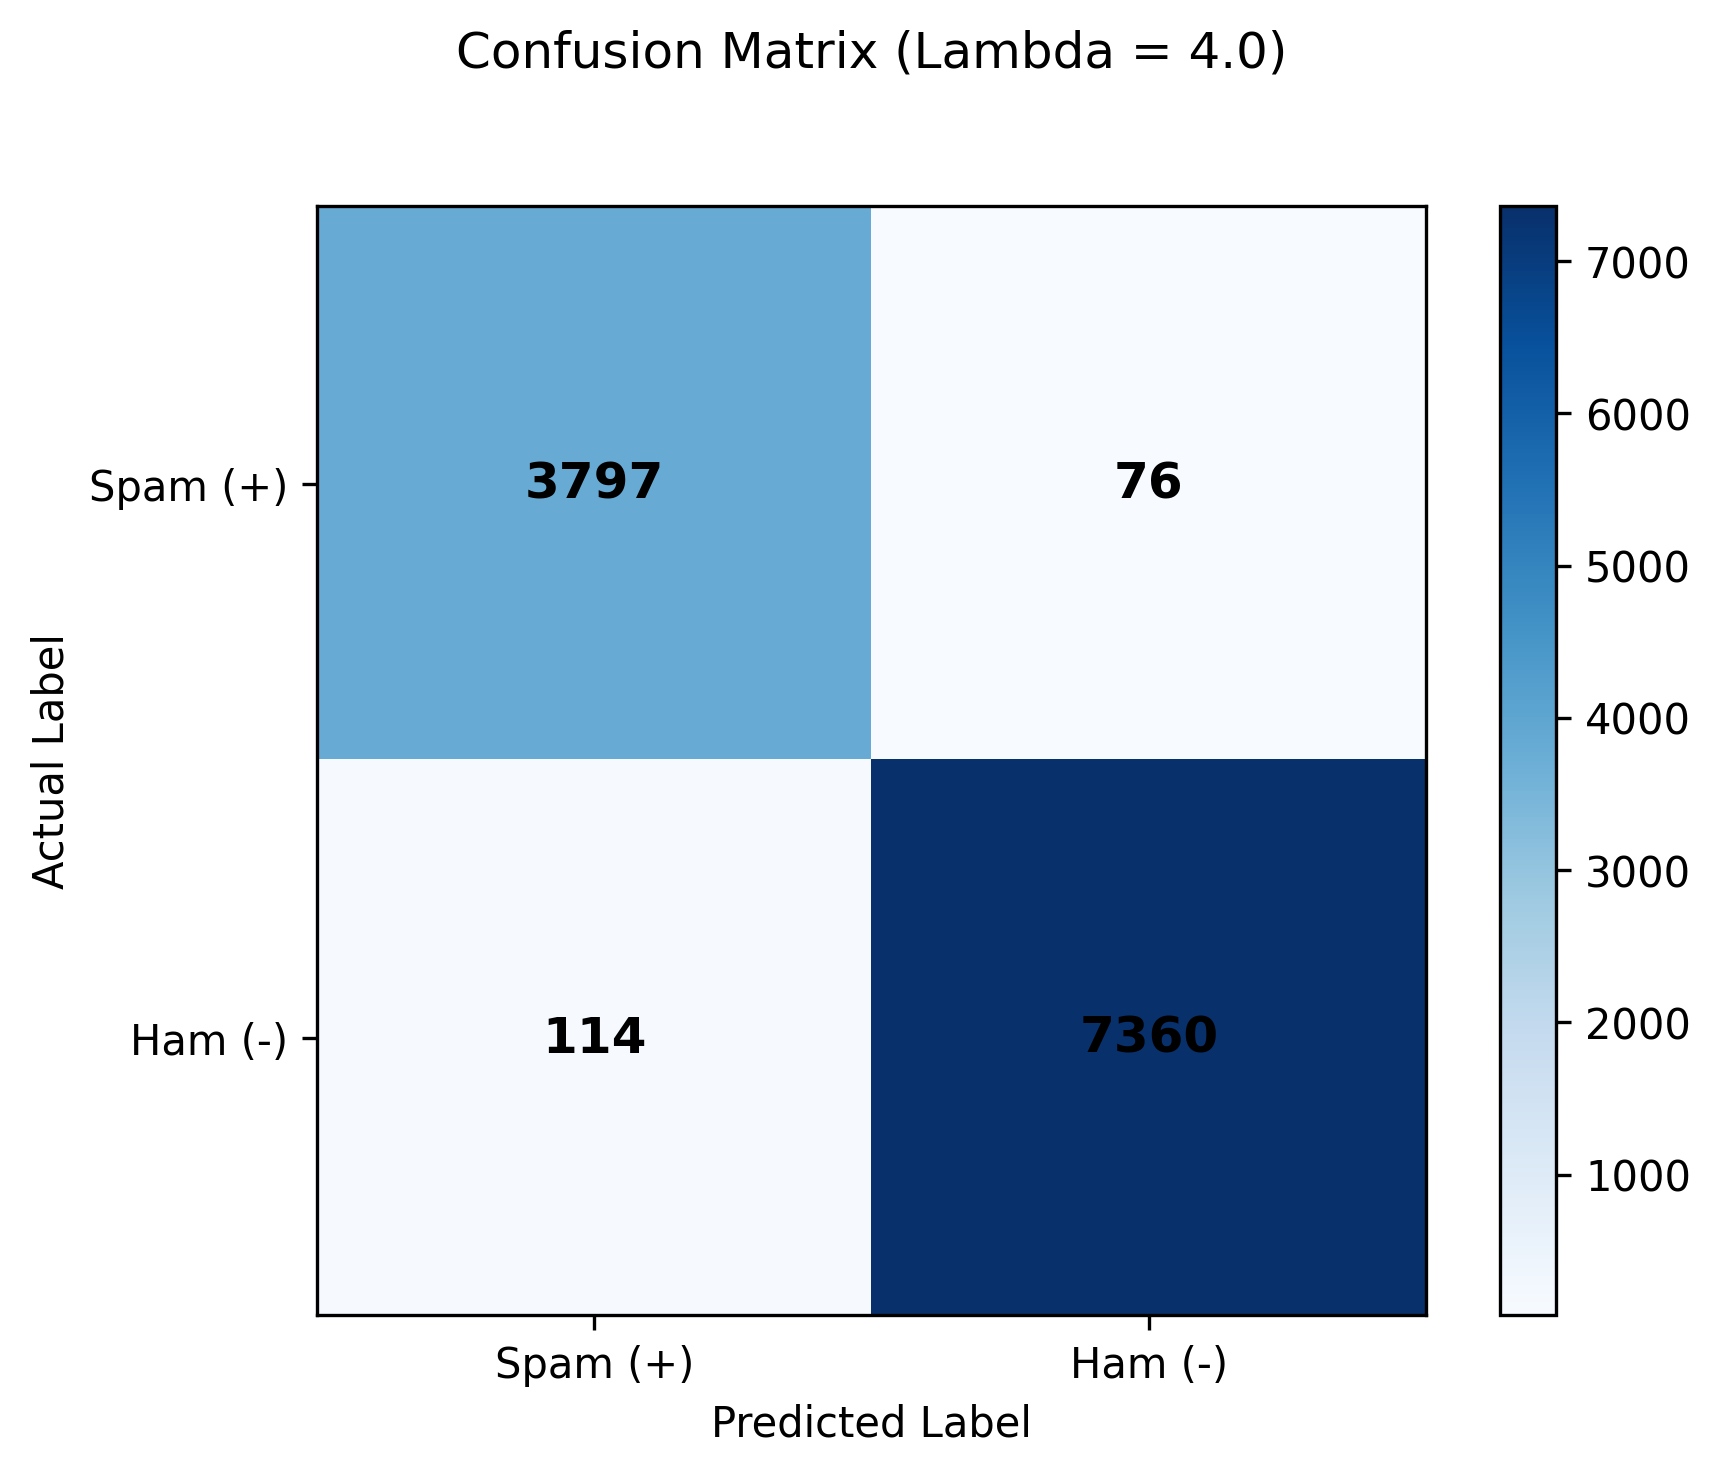
\includegraphics[width=0.475\textwidth]{results/confusion_matrix_lambda_4_0.png}
    \caption{Confusion Matrix for Lambda Smoothing with $\lambda = 4.0$.}
    \label{fig:confusion-matrix}
\end{figure}


\subsection{Mutual Information Results}

Table 3 shows the comparison of the performance metrics for the best model with Lambda smoothing ($\lambda = 4.0$) and the mutual information feature selection model with $k = 200$. We can see that the mutual information feature selection model has a much lower precision but a higher recall compared to the best Lambda smoothing model. We also compare it to the model with the best recall which outperforms the mutual information model in every metric.
\begin{table}[h]
\centering
\caption{Performance Comparison Across Different Model Configurations}
\begin{tabular}{lccc}
\toprule
Configuration & Precision & Recall & F1-Score \\
\midrule
Best Recall ($\lambda = 0.005$) & 0.8667 & 0.9990 & 0.9282 \\
Best F1 ($\lambda = 4.0$)      & 0.9709 & 0.9804 & 0.9756 \\
MI Top 200 ($\lambda = 4.0$)   & 0.5930 & 0.9853 & 0.7404 \\
\bottomrule
\end{tabular}
\end{table}

By increasing the number of relevant words by increasing $k$, we can improve the precision of the mutual information feature selection model. Figure 5 shows the precision and recall trends for different values of $k$. We can see that as $k$ increases, the precision increases while the recall decreases slightly.

\begin{figure}[h]
    \centering
    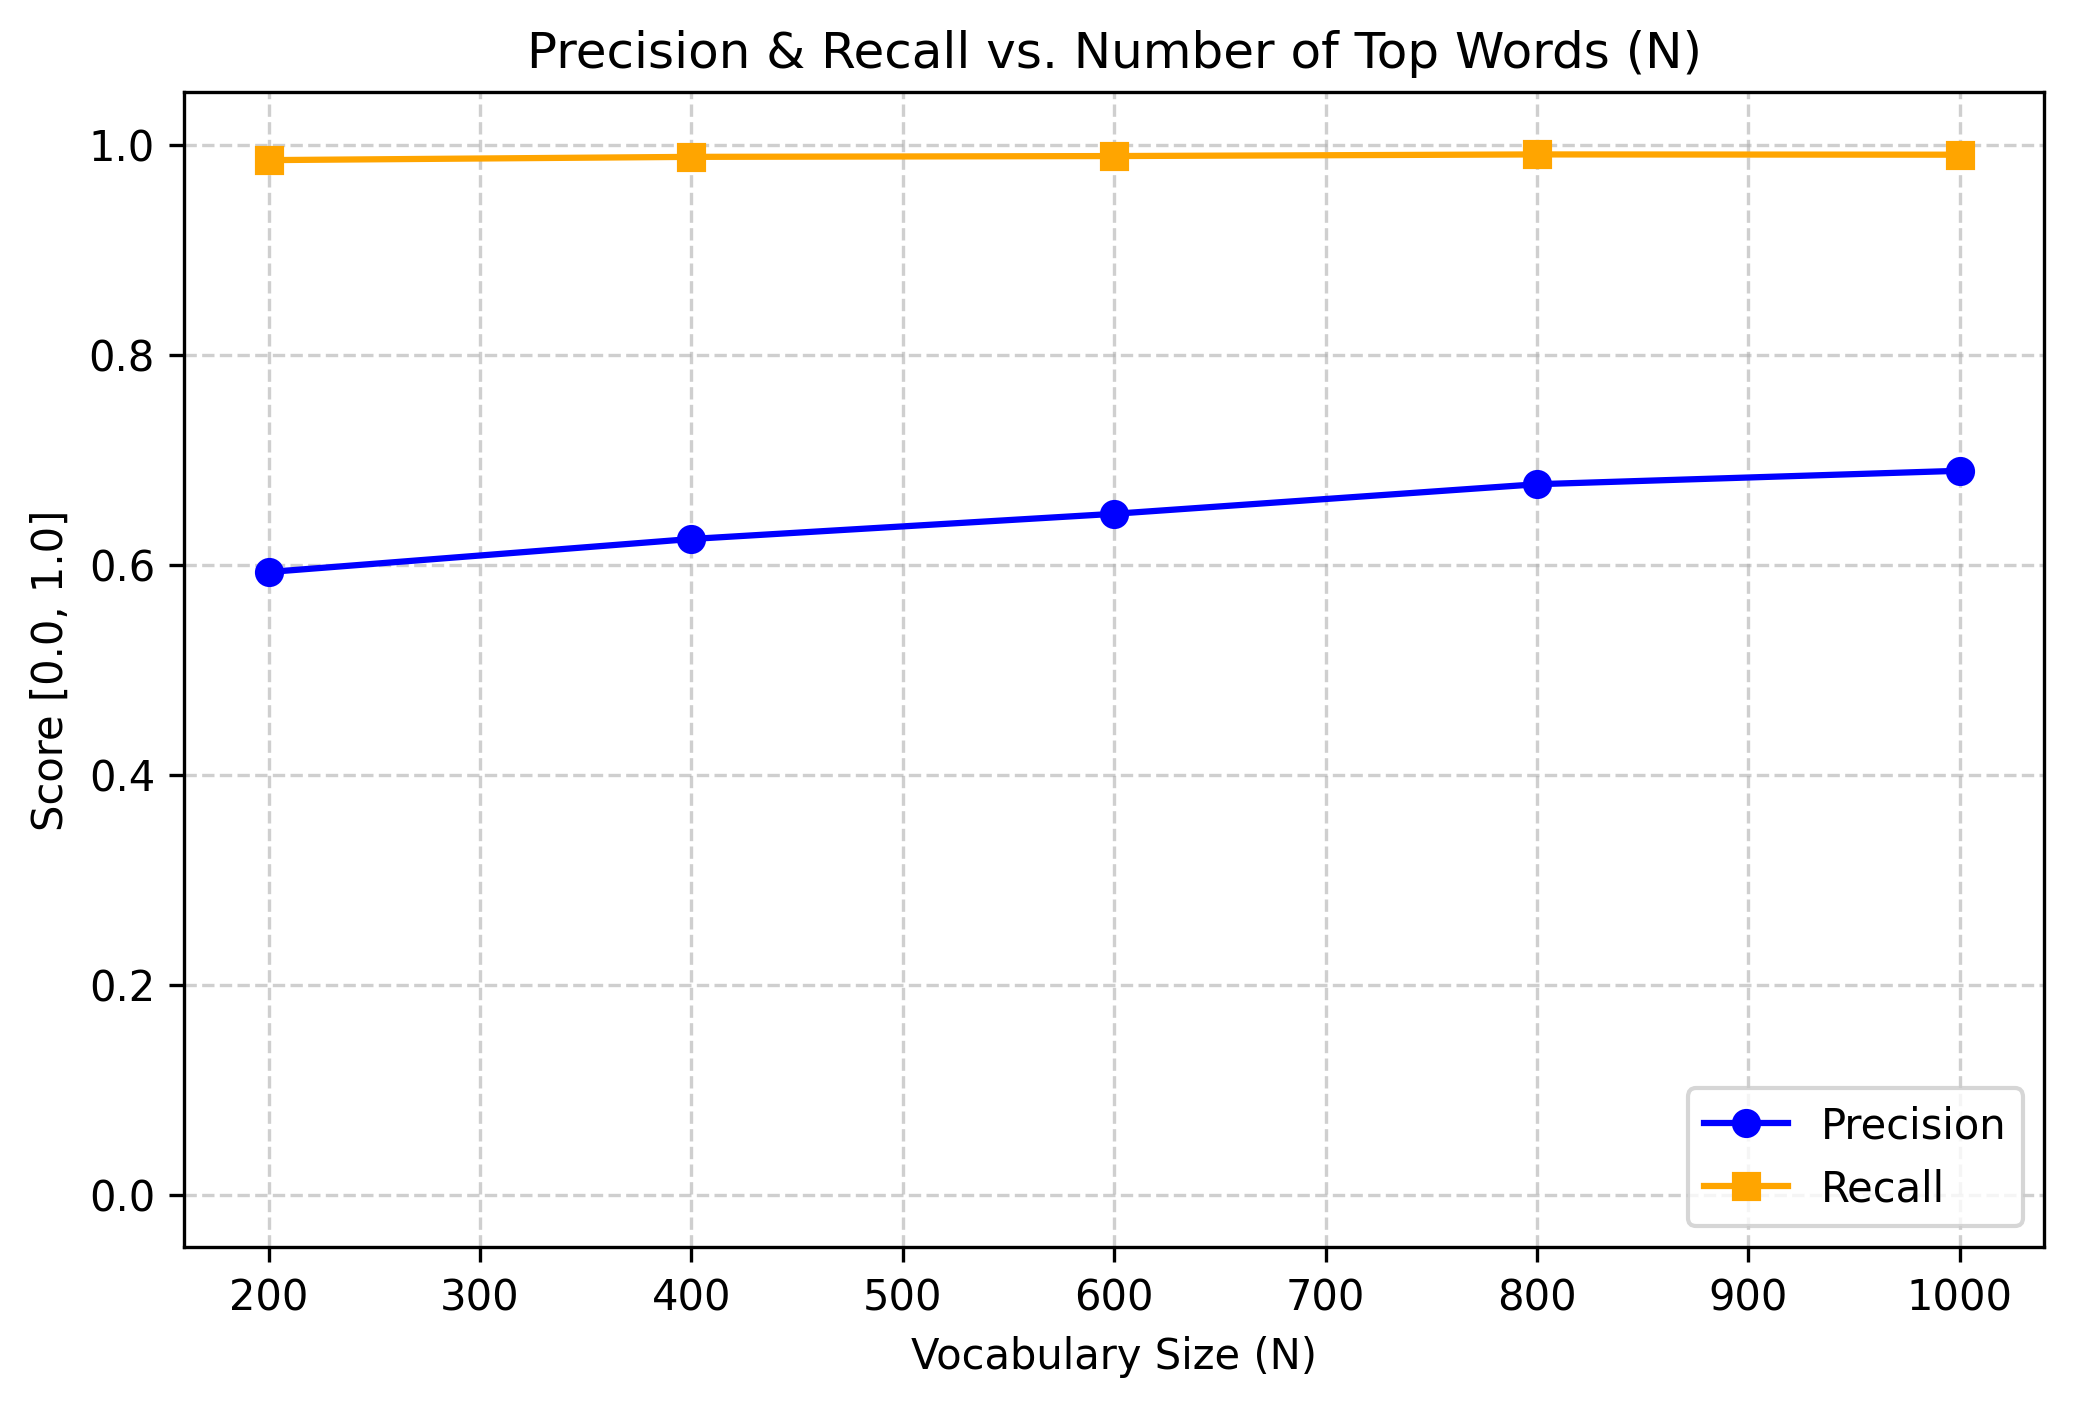
\includegraphics[width=0.475\textwidth]{results/mi_precision_recall_vs_n.png}
    \caption{Precision and Recall Trends vs k for Mutual Information Feature Selection.}
    \label{fig:mi-tradeoff}
\end{figure}

The time complexity and space complexity of the mutual information feature selection model is its main advantage over the previous models. While it performs worse, it is much more efficient in terms of computational and memory cost. Figure 6 and Figure 7 show the time complexity and space complexity trends for different values of $k$. We can see that as $k$ increases, the runtime increases almost linearly, while the memory consumption is almost negligible because it is just a mere fraction of the total vocabulary obtained from the training data.

\begin{figure}[h]
    \centering
    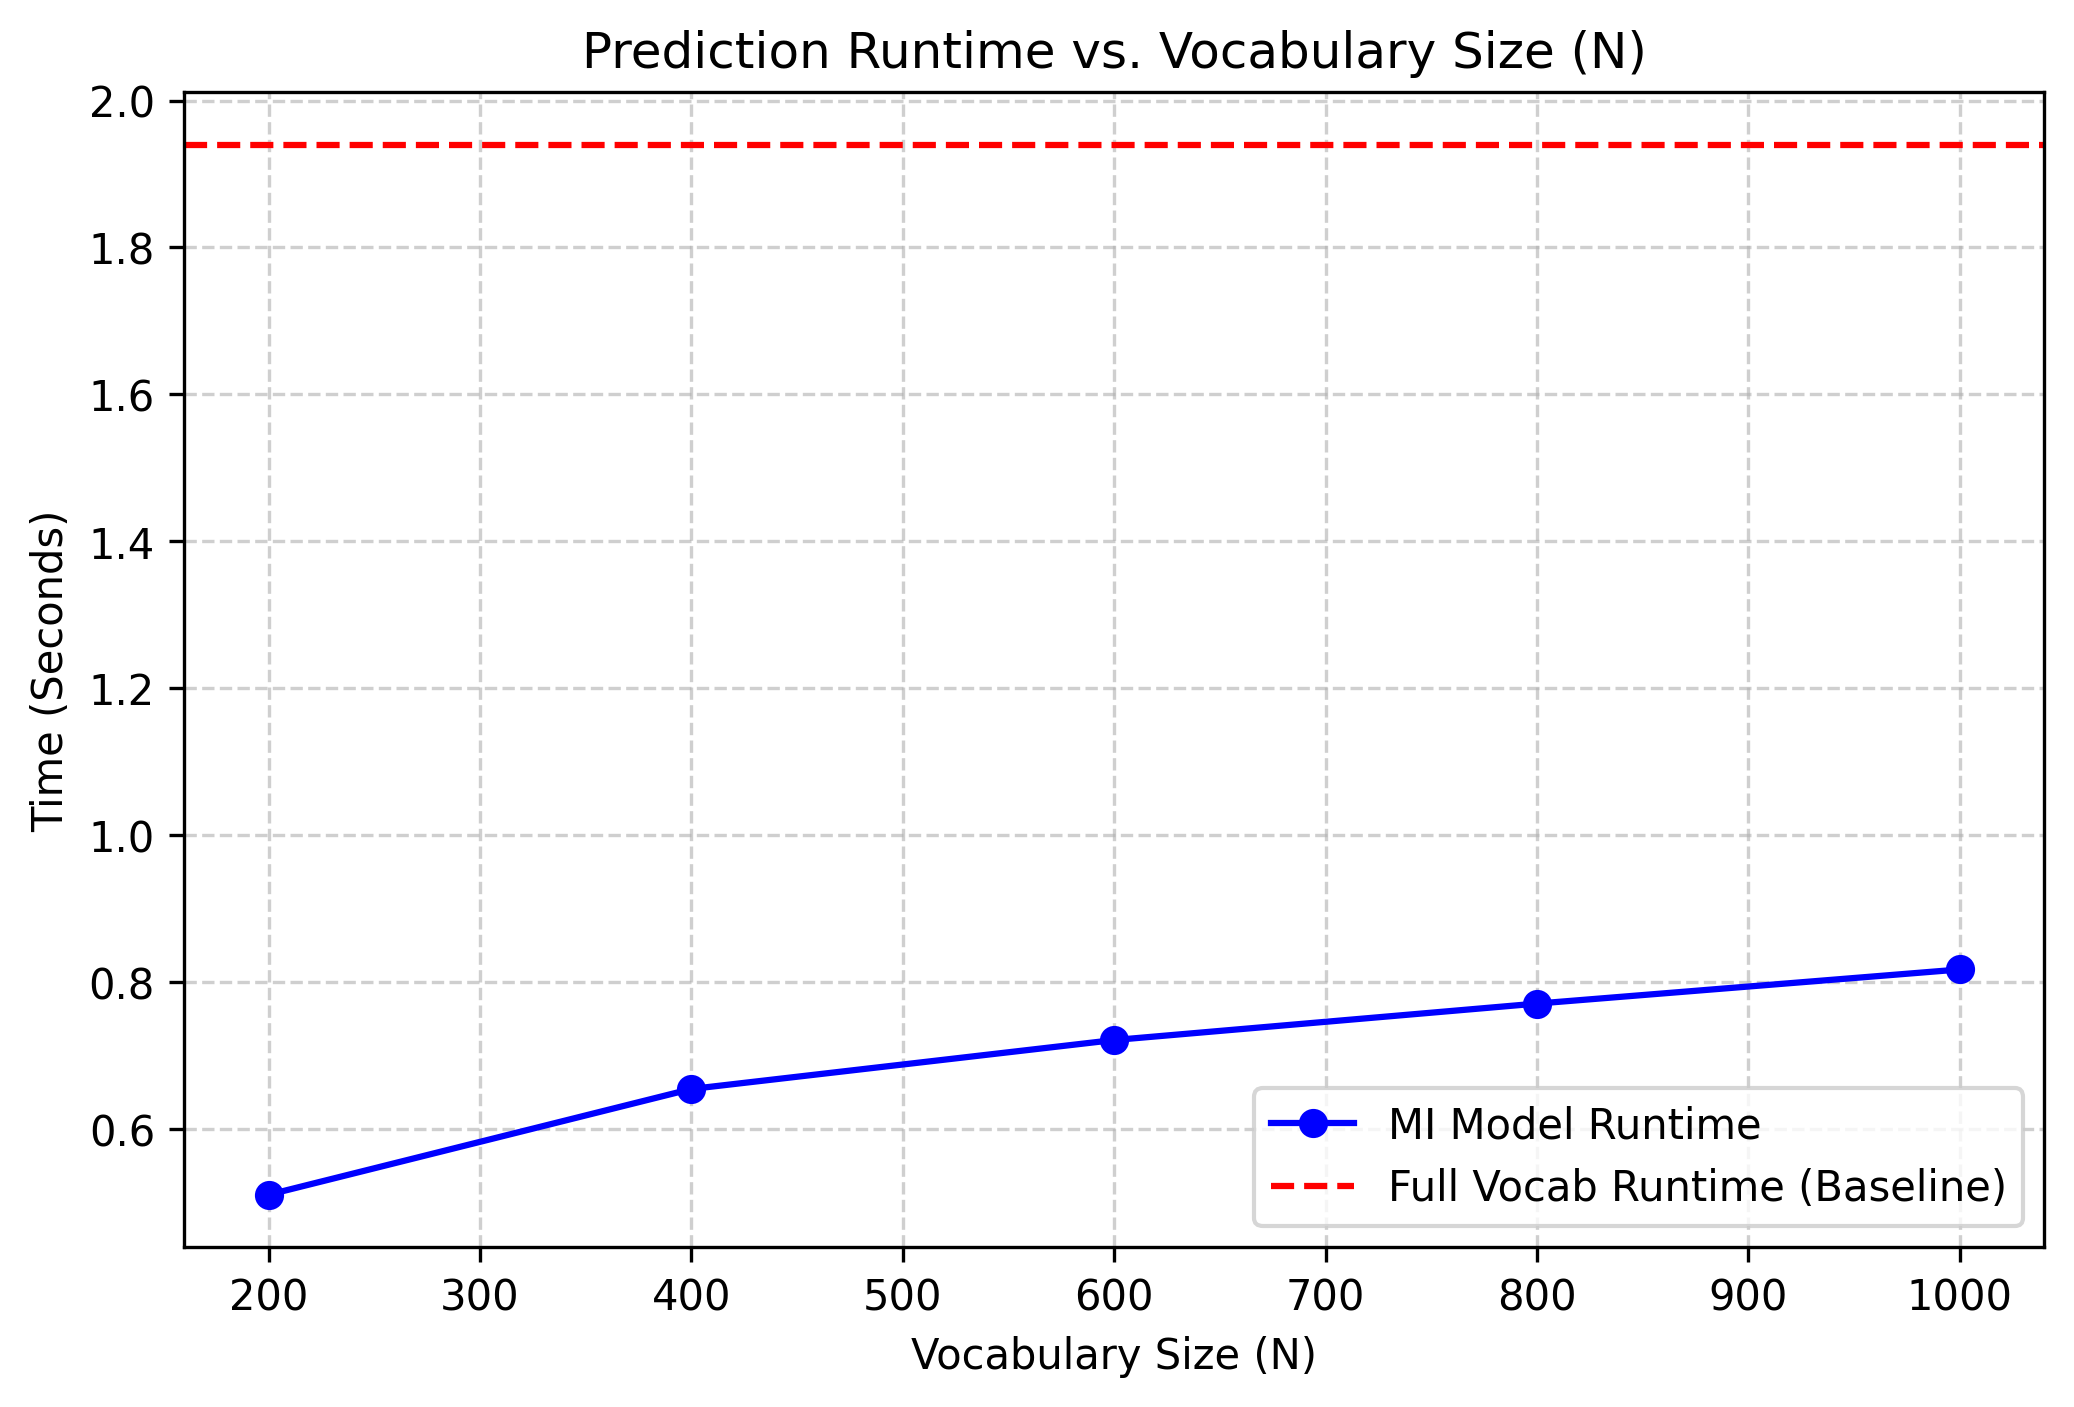
\includegraphics[width=0.475\textwidth]{results/time_complexity_plot.png}
    \caption{Time Complexity vs k of Mutual Information Feature Selection.}
    \label{fig:mi-time}
\end{figure}

\begin{figure}[h]
    \centering
    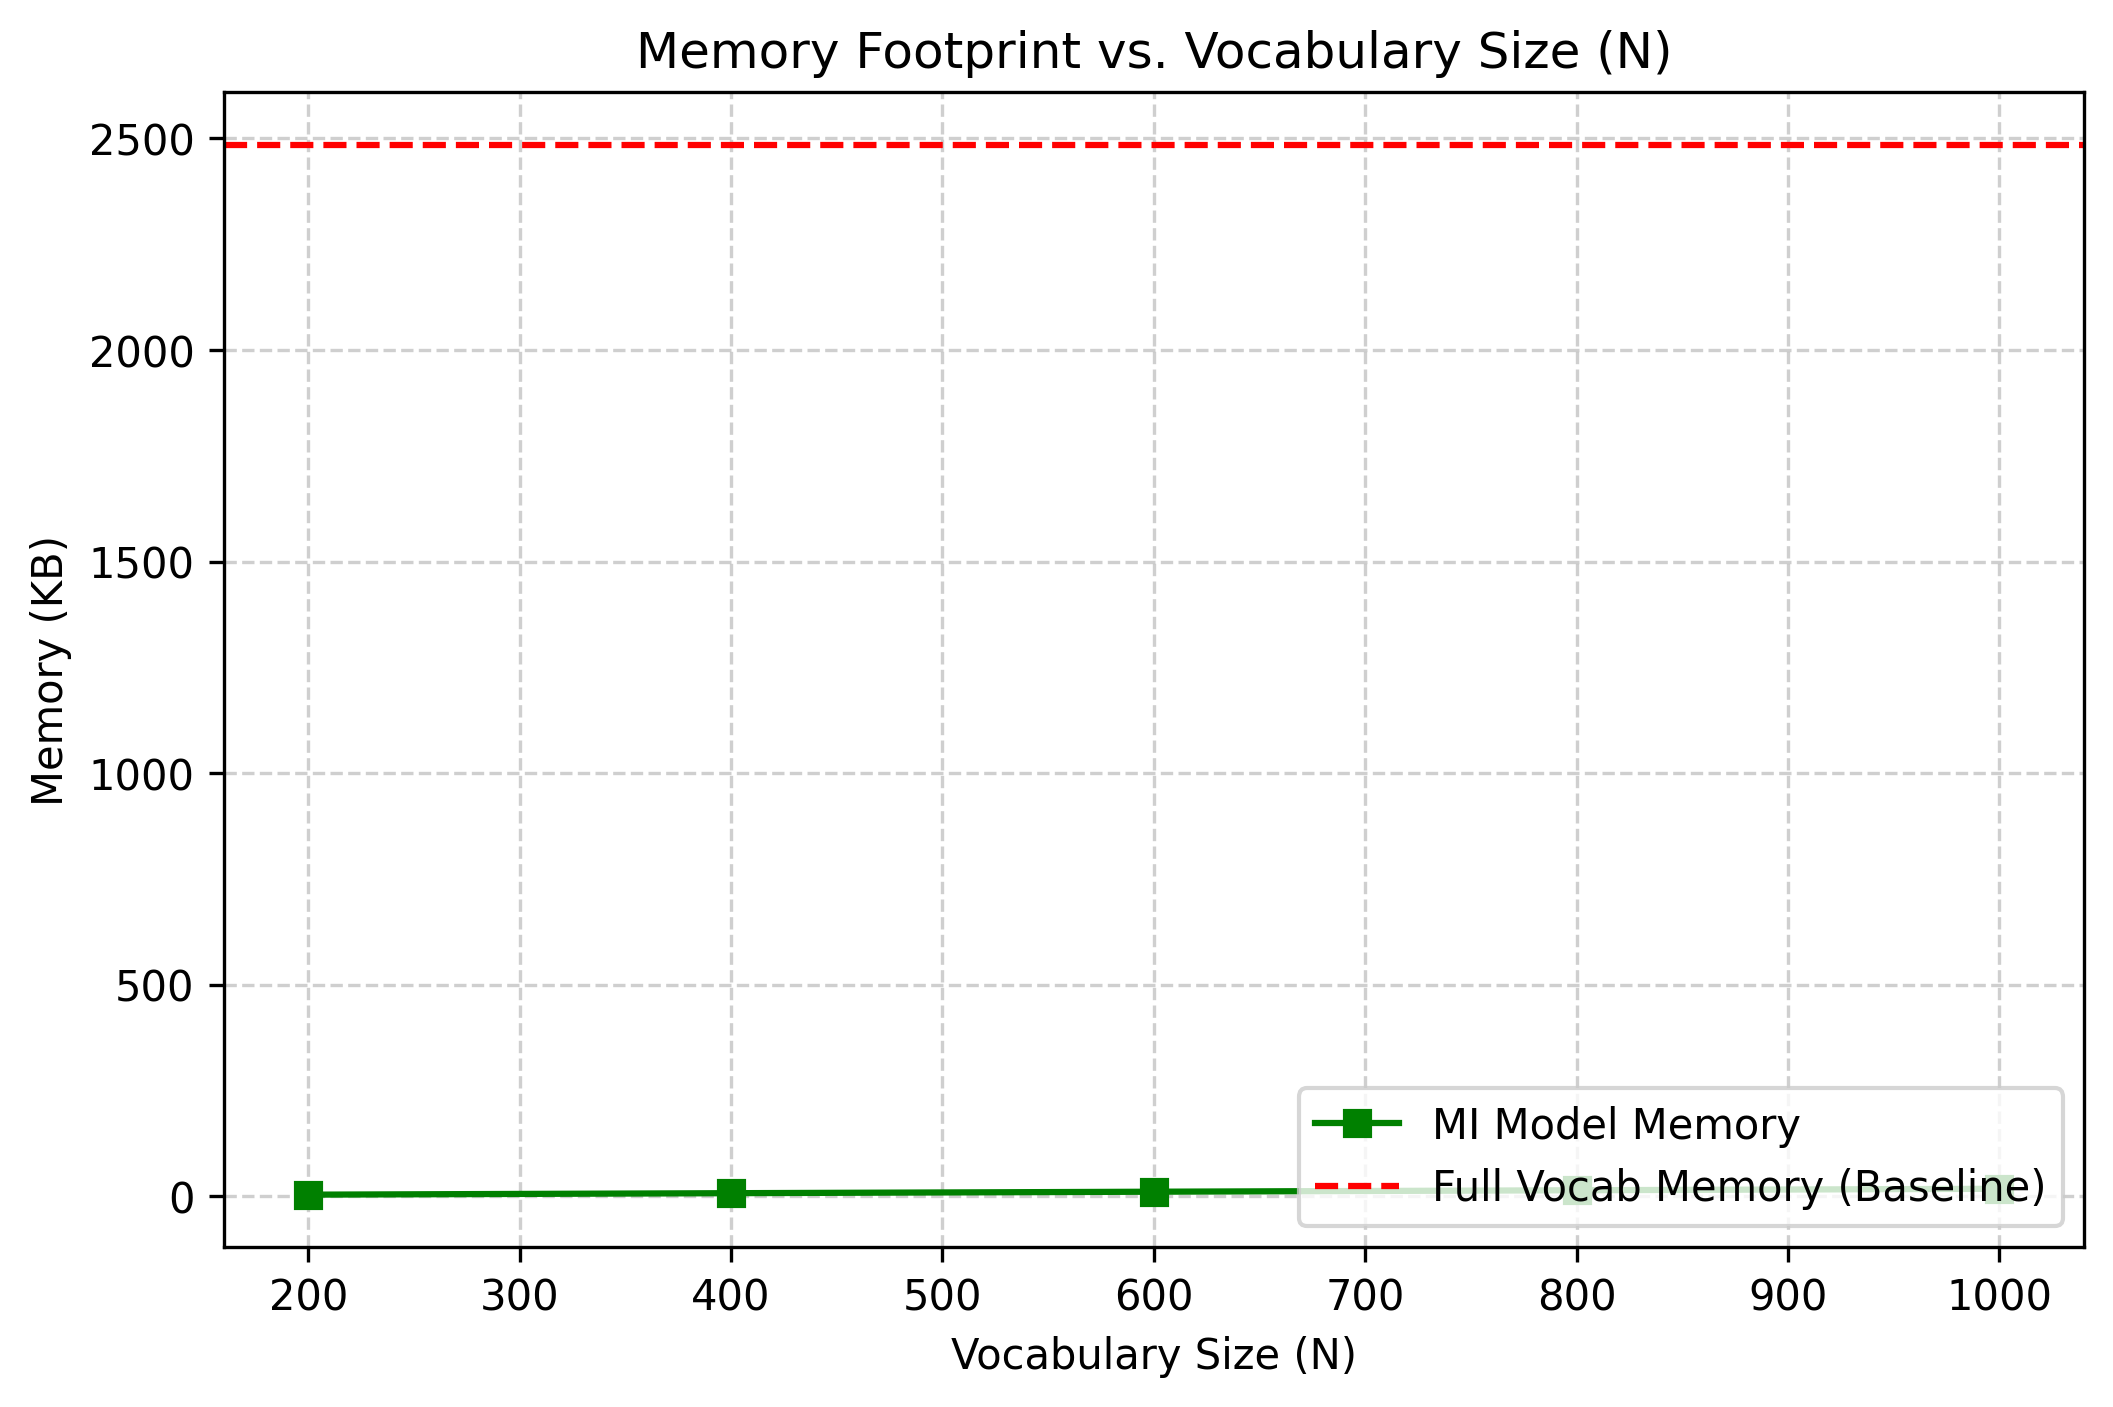
\includegraphics[width=0.475\textwidth]{results/space_complexity_plot.png}
    \caption{Space Complexity vs k of Mutual Information Feature Selection.}
    \label{fig:mi-space}
\end{figure}

\begin{table}[h]
\centering
\caption{Time Complexity Analysis: Runtime by Vocabulary Size}
\begin{tabular}{ccc}
\toprule
$N$ (Top Words) & Runtime (s) & Time Faster (\%) \\
\midrule
1000 & 0.817 & 57.89 \\
800  & 0.770 & 60.29 \\
600  & 0.721 & 62.84 \\
400  & 0.654 & 66.28 \\
200  & 0.510 & 73.70 \\
\bottomrule
\end{tabular}
\end{table}

\begin{table}[h]
\centering
\caption{Space Complexity Analysis: Memory Usage by Vocabulary Size}
\begin{tabular}{ccc}
\toprule
$N$ (Top Words) & Memory (KB) & Memory Saved (\%) \\
\midrule
1000 & 17.41 & 99.30 \\
800  & 13.93 & 99.44 \\
600  & 10.49 & 99.58 \\
400  & 7.02  & 99.72 \\
200  & 3.52  & 99.86 \\
\bottomrule
\end{tabular}
\end{table}

\section{Analysis and Discussion of Results}
\subsection{Effects of Lambda Smoothing}
The initial model is not ideal as it is not robust to unseen words in the test set. This behavior is expected as the model diverges when it encounters a word not present in the training set. With Lambda smoothing, the model performance increases substantially for all values of $\lambda$. This is because Lambda smoothing allows the model to assign a non-zero probability to unseen words, which prevents it from diverging and improves its generalization to the test set. However, as $\lambda$ increases, the precision increases while the recall decreases. This is because a larger $\lambda$ value allows the model to assign a non-zero probability to unseen words, which increases the precision but may also increase the number of false negatives, thus decreasing the recall. The intersection of the precision and recall curves is not enough to find the optimal $\lambda$ value produces the best model performance.

One way to find the best model is by looking at the F1-scores for different $\lambda$ values. We can see that the F1-score is highest at $\lambda = \{2.0,\ 4.0\}$, which suggests that this is the optimal $\lambda$ value for our model. This means that a moderate amount of smoothing is beneficial for our Naive Bayes classifier in terms of balancing precision and recall. Too little smoothing (small $\lambda$) produces a significantly higher recall but a much lower precision, while too much smoothing (large $\lambda$) produces a slightly higher precision but a much lower recall. This shows a tradeoff between precision and recall as we adjust the $\lambda$ value, and finding the optimal $\lambda$ value is crucial for achieving the best performance of the model.

We validate our results by using the receiver operating characteristic (ROC) curve to evaluate the performance of the model with the optimal $\lambda$ value. This will help validate our assumption that the model with $\lambda = \{2.0,\ 4.0\}$ has the best performance. As we can see, the models with the highest area under the curve (AUC) are the ones with $\lambda = \{2.0,\ 4.0\}$, which confirms our previous analysis. Among the tested values of $\lambda$, $\lambda = 1.0$ produces the same AUC as with our assumed best model, but it has a lower F1-score.

\subsection{Effects of Mutual Information}

The mutual information feature selection model is only able to capture the $k$ most relevant features that are correlated with the class labels, which increases the recall but may also increase the number of false positives, thus decreasing the precision. In fact, this model performs much worse than the model with the best recall, which is the model with $\lambda = 0.005$. This suggests that while mutual information feature selection can improve recall, it may not be the best approach for our spam filtering task as it significantly decreases precision and F1-score. 

Since we are using a significantly smaller vocabulary, the model is not able to capture all the relevant features that are necessary for accurate classification, which leads to a decrease in performance. However, by increasing the number of relevant words by increasing $k$, we can improve the precision of the mutual information feature selection model while maintaining a relatively high recall. The precision increases rapidly while the recall decreases slowly which is a good indicator that the model is performing better as we increase $k$.


\subsection{Performance vs Cost Tradeoff}

If we focus on efficiency and recall, the mutual information model with $k = 200$ is the best model as it has a much lower computational and memory cost while still maintaining a high recall. Table 4 and Table 5 show that the mutual information model with $k = 200$ saves a significant amount of time (73.70\%) and memory (99.86\%) compared to the best Lambda smoothing model, which is a huge advantage in terms of efficiency. 

The advantage of using a constant vocabulary size is that it allows us to control the computational and memory cost of the model, which can be beneficial in scenarios where resources are limited. However, this comes at the cost of performance as the model may not be able to capture all the relevant features necessary for accurate classification.


\section{Conclusion}
In this study, we developed a Naive Bayes classifier for spam filtering and investigated the effects of Lambda smoothing and mutual information feature selection on the performance of the model. We found that Lambda smoothing significantly improves the performance of the Naive Bayes classifier by preventing it from diverging when encountering unseen words. The optimal $\lambda$ value was found to be in the range of 2.0 to 4.0, which balances precision and recall effectively. The model with the best recall is the one with $\lambda = 0.005$, which can be useful in scenarios where minimizing false negatives is crucial. 

On the other hand, the mutual information feature selection model with $k = 200$ has a much lower computational and memory cost while still maintaining a high recall, making it a good choice for scenarios where efficiency is a concern. We can control the precision of the mutual information model by adjusting the value of $k$, which allows us to find a good balance between performance and cost. With a constant vocabulary size $k$, we can dedicate memory and computational resources to the model even if the training vocabulary size increases. 

While Naive Bayes classifier is simple, it offers a good baseline for spam filtering tasks. Overall, the choice of model configuration depends on the specific requirements of the spam filtering task and the tradeoffs between precision, recall, and efficiency.

\section{Recommendations}
We recommend improving the Naive Bayes classifier by implementing an n-gram model that buckets the words in the email into n-grams. This will allow the model to capture correlation among words and may improve its performance. With that, we recommend using the Kneser-Ney smoothing technique which is a more advanced smoothing technique that is commonly used in n-gram models for language modeling tasks.
\begin{thebibliography}{99}

\bibitem{Hovold2005}
Hovold, J. (2005). Naive Bayes spam filtering using word-position-based attributes. In \textit{Proceedings of the Second Conference on Email and Anti-Spam (CEAS 2005)} (pp. 1--8). Stanford University, CA, United States.

\bibitem{Vaswani2017}
Vaswani, A., Shazeer, N., Parmar, N., Uszkoreit, J., Jones, L., Gomez, A. N., Kaiser, Ł., \& Polosukhin, I. (2017). Attention is all you need. Advances in Neural Information Processing Systems, 30, 5998–6008.

\bibitem{Jurafsky2026a}
Jurafsky, D., \& Martin, J. H. (2026). N-gram language models. In Speech and Language Processing: An Introduction to Natural Language Processing, Computational Linguistics, and Speech Recognition with Language Models (3rd ed. draft, Jan 6, 2026).

\bibitem{Jurafsky2026b}
Jurafsky, D., \& Martin, J. H. (2026). Statistical constituency parsing. In Speech and Language Processing: An Introduction to Natural Language Processing, Computational Linguistics, and Speech Recognition with Language Models (3rd ed. draft, Jan 6, 2026).

\end{thebibliography}

\end{document}


